\documentclass[xcolor=dvipsnames]{beamer}


% ========
% EXTERNAL PACKAGES
% ========

\usepackage{amsmath,amssymb,mathtools}
\usepackage{tikz,tikz-cd,graphicx}
\usetikzlibrary{shapes.geometric,calc,patterns,decorations.pathreplacing,arrows,decorations.shapes,decorations.markings,math,arrows.meta}
\usepackage{bbm} % Required by \Id
\usepackage{mwe} % Defines \vcenter used to center an image within equation 

% ========
% MY PACKAGES
% ========

\providecommand{\MainFolder}{.}
\providecommand{\PackagesFolder}{\MainFolder/LatexPackages}
\providecommand{\GraphicsFolder}{\MainFolder/Graphics}

\usepackage{\PackagesFolder/my_math_1}

% ======
% BEAMER
% ======

\usetheme{boxes}
\usecolortheme{albatross}
\usefonttheme{structurebold}
% http://deic.uab.es/~iblanes/beamer_gallery/individual/boxes-albatross-structuresmallcapsserif.html

\setbeamerfont{itemize/enumerate body}{}
\setbeamerfont{itemize/enumerate subbody}{size=\normalsize}
\setbeamerfont{itemize/enumerate subsubbody}{size=\footnotesize}
\beamertemplatenavigationsymbolsempty % Remove navigation elements

% ======
% CUSTOM COMMANDS
% ======

\theoremstyle{plain}
\newtheorem{conjecture}{Conjecture} % Conjecture

\newcommand{\vcenterline}[1]{\begingroup
	\setbox0=\hbox{#1}
	\parbox{\wd0}{\box0}\endgroup} % Centers an element in line vertically

\renewcommand{\emph}[1]{{\itshape\color{pink}#1}}
\newcommand{\emphbf}[1]{{\bfseries\color{YellowGreen}#1}}

% =====
% TITLE
% =====

\title[Twisted $\IBLInfty$-structure]{IBL-Infinity Model of String Topology from Perturbative Chern-Simons Theory}
\author{Pavel H\'ajek}
\institute[University of Hamburg]{\emph{Department for Analysis and Differential Geometry, \\ University of Hamburg}}
\date{\emphbf{University of Augsburg, \\ $\argmin(\Abs{DDMM - 2019})$}}


\begin{document}

\begin{frame} % TITLEPAGE 
\titlepage
% Special day which minimizes distance to the year. There is at least one and maximally two such days every year. It will become non-unique in 2057 for the days 21.02. and 19.12.. Programming exercise for children. If what I wrote is wrong I give up immediately. Compute so that you can plan your wedding or funeral. I propose to celebrate "contemporary day" on these days. Because I have very advanced people in the classroom, so if you get bored, list some years when it is not unique. We can compare at the end. 
\end{frame}



\begin{frame}[fragile]{Bracket and cobracket in string topology}
\setlength{\leftmargini}{0pt}
\begin{itemize}
\item $\Sigma$ oriented surface (Goldman 86', Turaev 91'):
\newcommand{\ScaleFactor}{0.8}
\newcommand{\ParLength}{2.25cm}
\newcommand{\ParLengthII}{1.3cm}
\begin{align*}
\StringOp_2\left(
\parbox[c]{\ParLength}{
\begin{tikzpicture}[scale=\ScaleFactor]
	\def\rad{.8cm}
	\draw[thick,red,decoration={markings, mark=at position 0.25 with {\arrow{>}}},postaction={decorate}] ([shift=(0:\rad)]0,0) arc (0:360:\rad);  
	%\draw[green,thick,dotted] ([shift=(280:\rad)]0,0) arc (280:360:\rad);
	\draw[green,dashed,thick,decoration={markings, mark=at position 0.25 with {\arrow{>}}},postaction={decorate}] (1.5*\rad,0) circle (\rad);
	\end{tikzpicture}}
\right)
&=\parbox[c]{\ParLength}{
\begin{tikzpicture}[scale=\ScaleFactor]
	\def\rad{.8cm}
	\draw[blue,thick] ([shift=(90:\rad)]0,0) arc (90:360:\rad); %Big loop on the lft
    \draw[blue,thick] ([shift=(0:\rad)]0,0) arc (0:180:.25*\rad); %Small connecting loop
	\draw[blue,thick] ([shift=(180:\rad)]1.5*\rad,0) arc (180:450:\rad); %Big loop on the right
	\draw[blue,thick,decoration={markings, mark=at position 0.5 with {\arrow{<}}},
        postaction={decorate}] ([shift=(90:\rad)]0,0) to ([shift=(90:\rad)]1.5*\rad,0); %The oriented connecting line
\end{tikzpicture}}
\ -\ 
\parbox[c]{\ParLength}{
\begin{tikzpicture}[scale=\ScaleFactor]
	\def\rad{.8cm}
	\draw[blue,thick] ([shift=(0:\rad)]0,0) arc (0:270:\rad); %Big loop on the left
	\draw[blue,thick] ([shift=(180:\rad)]1.5*\rad,0) arc (180:360:.25*\rad); %Small connecting loop
	\draw[blue,thick] ([shift=(270:\rad)]1.5*\rad,0) arc (270:540:\rad); %Big loop on the right
	\draw[blue,thick,decoration={markings, mark=at position 0.5 with {\arrow{>}}},
        postaction={decorate}] ([shift=(270:\rad)]0,0) to ([shift=(270:\rad)]1.5*\rad,0);
\end{tikzpicture}}\\
\StringCoOp_2\left(\hspace{-.4em}
\parbox[c]{2.6cm}{
\begin{tikzpicture}[scale=\ScaleFactor]
	\def\rad{.8cm}
	\draw[blue,thick,decoration={markings, mark=at position 0.25 with {\arrow{>}}},
        postaction={decorate}] ([shift=(45:\rad)]0,0) arc (45:315:\rad);
	\draw[blue,thick,decoration={markings, mark=at position 0.25 with {\arrow{<}}},
        postaction={decorate}] ([shift=(-135:\rad)]2*\rad,0) arc (-135:135:\rad);
	\draw[blue,thick] (45:\rad) to[out=-45,in=135] ($(-135:\rad)+(2*\rad,0)$);
	\draw[blue,thick] (-45:\rad) to[out=45,in=225] ($(135:\rad)+(2*\rad,0)$);
\end{tikzpicture}}\right)
&=\parbox[c]{\ParLengthII}{
\begin{tikzpicture}[scale=\ScaleFactor]
\def\rad{.8cm}
\draw[red,thick,decoration={markings, mark=at position 0.25 with {\arrow{>}}},
        postaction={decorate}] (0,0) circle (\rad);
\end{tikzpicture}}\otimes
\parbox[c]{\ParLengthII}{
\begin{tikzpicture}[scale=\ScaleFactor]
\def\rad{.8cm}
\draw[green,dashed,thick,decoration={markings, mark=at position 0.25 with {\arrow{<}}},
        postaction={decorate}] (0,0) circle (\rad);
\end{tikzpicture}}\ -\ 
\parbox[c]{\ParLengthII}{
\begin{tikzpicture}[scale=\ScaleFactor]
\def\rad{.8cm}
\draw[green,dashed,thick,decoration={markings, mark=at position 0.25 with {\arrow{<}}},
        postaction={decorate}] (0,0) circle (\rad);
\end{tikzpicture}} \otimes
\parbox[c]{\ParLengthII}{
\begin{tikzpicture}[scale=\ScaleFactor]
\def\rad{.8cm}
\draw[red,thick,decoration={markings, mark=at position 0.25 with {\arrow{>}}},
        postaction={decorate}] (0,0) circle (\rad);
\end{tikzpicture}}
\end{align*}
\pause
\item Chas-Sullivan 99': $M^n$ oriented, $\Loop M$ loop space
\begin{align*}
\StringOp_2:&& \H^{\Sph{1}}_i(\Loop M) \otimes \H^{\Sph{1}}_j(\Loop M) & \longrightarrow \H^{\Sph{1}}_{i+j + 2 - n}(\Loop M) \\
\StringCoOp_2:&&  \bar{\H}^{\Sph{1}}_k(\Loop M) &\longrightarrow\!\!\!\!\bigoplus_{i + j = k + 2 - n}\!\!\!\bar{\H}^{\Sph{1}}_i(\Loop M) \otimes \bar{\H}^{\Sph{1}}_j(\Loop M)
\end{align*}
\end{itemize}
% The generic picture are immersed loops with transverse double-points. Explain the picture. The construction of Chas-Sullivan follows the same picture just the intersection points are taken from transverse intersection of smooth parameter spaces of points on the loops. Hence the degree 2-n. To formulate it precisely one needs geometric homology theory and homotop to the   generic situation. Therefore, the operations are defined on homology.
\end{frame}

\begin{frame}{IBL-algebra}
\begin{theorem}[Chas-Sullivan 04']
$(\bar{\H}^{\Sph{1}}(\Loop M), \StringOp_2, \StringCoOp_2)$ is an \emph{involutive bi-Lie algebra} of degree $2-n$.
\end{theorem}\pause

{ \begingroup \allowdisplaybreaks
\def\dist{0.25} %distance between two surfaces
  \def\rad{0.4} % radius of bdd
  \def\ecc{0.1} % eccentricity of bdd
  \def\hght{1} % height of surfaces
  \def\dif{1.1} % distance of two circles
  \def\difbig{1.5*\dif} % distance of two circles
  \def\radO{\rad} % radius of bdd
  \def\eccO{\ecc} % eccentricity of bdd
  \def\hghtO{2*\hght+\dist} % height of surfaces
  \def\difO{\dif} % distance of two circles
  \def\gencanc{0.05} % legth of extra line in genus
  \def\genecc{20} % eccentricity of genus
  \def\genrad{0.3} % radius of genus
  \newcommand{\PicScaling}{.8}
\begin{align*}
0 & =\quad\vcenterline{%auto-ignore
\begin{tikzpicture}[scale=\PicScaling]
  % Sphere
  
  \coordinate (P1) at (0,0);
  \coordinate (P2) at (-0.5*\difbig,\hght);
  \coordinate (P3) at ($(0.5*\difbig,\hght)$);

  \coordinate (P4) at ($(P2)+(0,\dist)$);
  \coordinate (P5) at ($(P4)+(-0.5*\dif,\hght)$);
  \coordinate (P6) at ($(P4)+(0.5*\dif,\hght)$);


  \coordinate (P7) at ($(P6)+(0,-\hght)$);
  \coordinate (P8) at ($(P3)+(0,\dist)$);
  \coordinate (P9) at ($(P8)+(0,\hght)$);

%Pair of pants
  
  \draw (P1) arc (180:360:{\rad} and {\ecc});
  \draw[dashed] (P1) arc (180:0:{\rad} and {\ecc});
  
   \draw (P3) arc (180:360:{\rad} and {\ecc});
  \draw (P3) arc (180:0:{\rad} and {\ecc});
  
  \draw (P2) arc (180:360:{\rad} and {\ecc});
  \draw (P2) arc (180:0:{\rad} and {\ecc});
  
 \draw (P2) to[out=270,in=90] (P1);
 \draw ($(P3)+(2*\rad,0)$) to[out=270,in=90] ($(P1)+(2*\rad,0)$);
 \draw ($(P2)+(2*\rad,0)$) to[out=270,in=270] (P3); 
 
% Maurer Cartan


 
  \draw (P4) arc (180:360:{\rad} and {\ecc});
  \draw[dashed] (P4) arc (180:0:{\rad} and {\ecc});
  
   \draw (P6) arc (180:360:{\rad} and {\ecc});
  \draw (P6) arc (180:0:{\rad} and {\ecc});
  
  \draw (P5) arc (180:360:{\rad} and {\ecc});
  \draw (P5) arc (180:0:{\rad} and {\ecc});
  
 \draw (P5) to[out=270,in=90] (P4);
 \draw ($(P6)+(2*\rad,0)$) to[out=270,in=90] ($(P4)+(2*\rad,0)$);
 \draw ($(P5)+(2*\rad,0)$) to[out=270,in=270] (P6); 

% \draw (P4) arc (180:360:{\rad} and {\ecc});
% \draw[dashed] (P4) arc (180:0:{\rad} and {\ecc});
% 
% \draw (P5) arc (180:360:{\rad} and {\ecc});
% \draw[dashed] (P5) arc (180:0:{\rad} and {\ecc});
% 
% \draw ($(P5)+(2*\rad,0)$) to[out=90,in=90] (P4);
% 
% \draw (P5) to[out=90,in=180] ($0.5*(P4)+(\rad,0)+0.5*(P5)+(0,\hght)$) to[out=0,in=90] ($(P4)+(2*\rad,0)$);

% Labels 
 
% \node at ($(P1)+(\rad,0.42*\hght)$) {$\OPQ_{210}^\PMC$};
% \node at ($(P4)+(\rad,0.5*\hght)$) {$\OPQ_{210}^\PMC$};
% \node at ($0.5*(P4)+(\rad,0)+0.5*(P5)+(0,0.5*\hght)$) {$\PMC_{20}$};

% Cylinders 

% \draw (P6) arc (180:360:{\rad} and {\ecc});
% \draw (P6) arc (180:0:{\rad} and {\ecc});  
% \draw (P7) arc (180:360:{\rad} and {\ecc});
% \draw[dashed] (P7) arc (180:0:{\rad} and {\ecc});
% \draw (P6) -- (P7);
% \draw ($(P6)+(2*\rad,0)$) -- ($(P7)+(2*\rad,0)$);
% 
 
 \draw (P9) arc (180:360:{\rad} and {\ecc});
 \draw (P9) arc (180:0:{\rad} and {\ecc});  
 \draw (P8) arc (180:360:{\rad} and {\ecc});
 \draw[dashed] (P8) arc (180:0:{\rad} and {\ecc});
 \draw (P8) -- (P9);
 \draw ($(P8)+(2*\rad,0)$) -- ($(P9)+(2*\rad,0)$);
  
\end{tikzpicture}} & 0&=\quad \vcenterline{%auto-ignore
\begin{tikzpicture}[scale=\PicScaling]
  
  \coordinate (P1) at (0,0);
  \coordinate (P2) at ($(P1) + (-0.5*\dif,\hght)$);  
  \coordinate (P3) at ($(P1) + (0.5*\dif,\hght)$);
  
  \coordinate (P4) at (0,-\dist);
  \coordinate (P5) at ($(P4) + (-0.5*\dif,-\hght)$);  
  \coordinate (P6) at ($(P4) + (0.5*\dif,-\hght)$);
  
  \draw (P1) to[out=90, in=-90] (P2);
  \draw ($(P1)+(2*\rad,0)$) to[out=90, in=-90] ($(P3)+(2*\rad,0)$);  
  \draw ($(P2)+(2*\rad,0)$) to[out=-90,in=-90] (P3);
 
   \draw (P4) to[out=-90, in=90] (P5);
  \draw ($(P4)+(2*\rad,0)$) to[out=-90, in=90] ($(P6)+(2*\rad,0)$);  
  \draw ($(P5)+(2*\rad,0)$) to[out=90,in=90] (P6); 
  
  \draw (P1) arc (180:360:{\rad} and {\ecc});
  \draw[dashed] (P1) arc (180:0:{\rad} and {\ecc});
  \draw (P5) arc (180:360:{\rad} and {\ecc});
  \draw[dashed] (P5) arc (180:0:{\rad} and {\ecc});
  \draw (P6) arc (180:360:{\rad} and {\ecc});
  \draw[dashed] (P6) arc (180:0:{\rad} and {\ecc});
 
  \draw (P2) arc (180:360:{\rad} and {\ecc});
  \draw (P2) arc (180:0:{\rad} and {\ecc});
  \draw (P3) arc (180:360:{\rad} and {\ecc});
  \draw (P3) arc (180:0:{\rad} and {\ecc});
  \draw (P4) arc (180:360:{\rad} and {\ecc});
  \draw (P4) arc (180:0:{\rad} and {\ecc}); 
 
% \node at ($(P1)+(\rad,0.5*\hght)$) {$\OPQ_{210}^\PMC$};
% \node at ($0.5*(P5)+(\rad,0)+0.5*(P6)+(0,0.5*\hght)$) {$\OPQ_{120}^\PMC$};

\end{tikzpicture}} +\quad \vcenterline{%auto-ignore
\begin{tikzpicture}[scale=\PicScaling]

 \coordinate (P1) at (0,0);
 \coordinate (P2) at ($(P1)+(0.5*\dif,\hght)$);
 \coordinate (P3) at ($(P1) + (\dif,0)$);
 \coordinate (P4) at ($(P3) + (0,-\dist)$);
 \coordinate (P5) at ($(P4) + (0.5*\dif,-\hght)$);
 \coordinate (P6) at ($(P4) + (\dif,0)$);
 
 \draw (P1) to[out=90,in=-90] (P2);
 \draw ($(P1)+(2*\rad,0)$) to[out=90,in=90] (P3);
 \draw ($(P2)+(2*\rad,0)$) to[out=-90,in=90] ($(P3)+(2*\rad,0)$); 
 \draw (P4) to[out=-90,in=90] (P5);
 \draw ($(P4)+(2*\rad,0)$) to[out=-90,in=-90] (P6);
 \draw ($(P5)+(2*\rad,0)$) to[out=90,in=-90] ($(P6)+(2*\rad,0)$);
 
 
  \draw (P1) arc (180:360:{\rad} and {\ecc});
  \draw[dashed] (P1) arc (180:0:{\rad} and {\ecc});
  \draw (P3) arc (180:360:{\rad} and {\ecc});
  \draw[dashed] (P3) arc (180:0:{\rad} and {\ecc});
  \draw (P5) arc (180:360:{\rad} and {\ecc});
  \draw[dashed] (P5) arc (180:0:{\rad} and {\ecc});
 
 
  \draw (P2) arc (180:360:{\rad} and {\ecc});
  \draw (P2) arc (180:0:{\rad} and {\ecc});
  \draw (P4) arc (180:360:{\rad} and {\ecc});
  \draw (P4) arc (180:0:{\rad} and {\ecc});
  \draw (P6) arc (180:360:{\rad} and {\ecc});
  \draw (P6) arc (180:0:{\rad} and {\ecc});
  
%    \node at ($(P2)+(\rad,-0.5*\hght)$) {$\OPQ_{120}^\PMC$};
% \node at ($(P5)+(\rad,0.5*\hght)$) {$\OPQ_{210}^\PMC$};
 
 \coordinate (P7) at ($(P1)+(0,-\dist)$);
 \coordinate (P8) at ($(P7)+(0,-\hght)$);
 \coordinate (P9) at ($(P6)+(0,\dist)$);
 \coordinate (P10) at ($(P9)+(0,\hght)$);
 
 \draw (P7)--(P8);
 \draw ($(P7)+(2*\rad,0)$)--($(P8)+(2*\rad,0)$);
 \draw (P9)--(P10);
 \draw ($(P9)+(2*\rad,0)$)--($(P10)+(2*\rad,0)$);
 
 
\draw (P8) arc (180:360:{\rad} and {\ecc});
\draw[dashed] (P8) arc (180:0:{\rad} and {\ecc});
\draw (P9) arc (180:360:{\rad} and {\ecc});
\draw[dashed] (P9) arc (180:0:{\rad} and {\ecc});
\draw (P7) arc (180:360:{\rad} and {\ecc});
\draw (P7) arc (180:0:{\rad} and {\ecc});
\draw (P10) arc (180:360:{\rad} and {\ecc});
\draw (P10) arc (180:0:{\rad} and {\ecc}); 
 
\end{tikzpicture}}\\[1ex] 
0&=\quad \vcenterline{%auto-ignore
\begin{tikzpicture}[scale=\PicScaling]
  \coordinate (P1) at (0,\hght);
  \coordinate (P2) at (-0.5*\difO,0);
  \coordinate (P3) at (0.5*\difO,0);
  \coordinate (P4) at ($(P1) + (-0.5*\difbig,\dist+\hght)$);
  \coordinate (P5) at ($(P4)+(-0.5*\difbig,-\hght)$);
  \coordinate (P6) at ($(P4) + (0.5*\difbig,-\hght)$);
%Pair of pants 
 
%  \draw (P5) arc (180:360:{\radO} and {\eccO});
%  \draw (P5) arc (180:0:{\radO} and {\eccO});
%  \draw (P4) arc (180:360:{\radO} and {\eccO});
%  \draw[dashed] (P4) arc (180:0:{\radO} and {\eccO});
%  \draw (P4) -- (P5);
%  \draw ($(P4)+(2*\rad0,0)$) -- ($(P5)+(2*\rad0,0)$);
  
  \draw (P1) arc (180:360:{\radO} and {\eccO});
  \draw (P1) arc (180:0:{\radO} and {\eccO});
  
   \draw (P3) arc (180:360:{\radO} and {\eccO});
  \draw[dashed] (P3) arc (180:0:{\radO} and {\eccO});
  
  \draw (P2) arc (180:360:{\radO} and {\eccO});
  \draw[dashed] (P2) arc (180:0:{\radO} and {\eccO});
  
 \draw (P2) to[out=90,in=270] (P1);
 \draw ($(P3)+(2*\radO,0)$) to[out=90,in=270] ($(P1)+(2*\radO,0)$);
 \draw ($(P2)+(2*\radO,0)$) to[out=90,in=90] (P3); 
 
 
 
  \draw (P4) arc (180:360:{\radO} and {\eccO});
  \draw (P4) arc (180:0:{\radO} and {\eccO});
  
   \draw (P6) arc (180:360:{\radO} and {\eccO});
  \draw[dashed] (P6) arc (180:0:{\radO} and {\eccO});
  
  \draw (P5) arc (180:360:{\radO} and {\eccO});
  \draw[dashed] (P5) arc (180:0:{\radO} and {\eccO});
  
 \draw (P5) to[out=90,in=270] (P4);
 \draw ($(P6)+(2*\radO,0)$) to[out=90,in=270] ($(P4)+(2*\radO,0)$);
 \draw ($(P5)+(2*\radO,0)$) to[out=90,in=90] (P6); 
 
% Labels 
 
% \node at ($0.5*(P2)+(\radO,0)+0.5*(P3)+(0,0.21*\hghtO-.7*\dist)$) {$\OPQ_{120}^\PMC$};
% 
%  \node at ($0.5*(P5)+(\radO,0)+0.5*(P6)+(0,0.21*\hghtO-.7*\dist)$) {$\OPQ_{120}^\PMC$};
  

\coordinate (P7) at ($(P5) + (0,-\dist)$);
\coordinate (P8) at ($(P7) + (0,-\hght)$);
\draw (P7)--(P8);
\draw ($(P7)+(2*\rad,0)$)--($(P8)+(2*\rad,0)$);

  \draw (P7) arc (180:360:{\radO} and {\eccO});
  \draw (P7) arc (180:0:{\radO} and {\eccO});
  
   \draw (P8) arc (180:360:{\radO} and {\eccO});
  \draw[dashed] (P8) arc (180:0:{\radO} and {\eccO});


\end{tikzpicture}} & 0& =\quad \vcenterline{%auto-ignore
\begin{tikzpicture}[scale=\PicScaling]

\coordinate (P1) at (0,0);
\coordinate (P2) at (-0.5*\dif,-\hght);
\coordinate (P3) at (0.5*\dif,-\hght);

\coordinate (P4) at ($(P2)+(0,-\dist)$);
\coordinate (P5) at ($(P3)+(0,-\dist)$);
\coordinate (P6) at ($(P4)+(0.5*\dif,-\hght)$);

\draw (P1) to[out=-90,in=90] (P2);
\draw ($(P1)+(2*\rad,0)$) to[out=-90,in=90] ($(P3)+(2*\rad,0)$);
\draw ($(P2)+(2*\rad,0)$) to[out=90,in=90] (P3);

\draw ($(P4)+(2*\rad,0)$) to[out=-90,in=-90] (P5);
\draw (P4) to[out=-90,in=90] (P6);
\draw ($(P5)+(2*\rad,0)$) to[out=-90,in=90] ($(P6)+(2*\rad,0)$);

 
\draw (P1) arc (180:360:{\rad} and {\ecc});
\draw (P1) arc (180:0:{\rad} and {\ecc});
\draw (P2) arc (180:360:{\rad} and {\ecc});
\draw[dashed] (P2) arc (180:0:{\rad} and {\ecc});
\draw (P3) arc (180:360:{\rad} and {\ecc});
\draw[dashed] (P3) arc (180:0:{\rad} and {\ecc});
\draw (P4) arc (180:360:{\rad} and {\ecc});
\draw (P4) arc (180:0:{\rad} and {\ecc}); 
\draw (P5) arc (180:360:{\rad} and {\ecc});
\draw (P5) arc (180:0:{\rad} and {\ecc}); 
\draw (P6) arc (180:360:{\rad} and {\ecc});
\draw[dashed] (P6) arc (180:0:{\rad} and {\ecc}); 

%\node at ($(P1)+(\rad,-0.5*\hght)$) {$\OPQ_{120}^\PMC$};
%\node at ($(P6)+(\rad,0.5*\hght)$) {$\OPQ_{210}^\PMC$};

\end{tikzpicture}}
\end{align*}
\endgroup}
% It is standard homology, or relative to one point, or relative to constant loops. The correct version is in the paper of Kai on Poincare duality in Rabinowitz-Floer homology.
\end{frame}

\begin{frame}{Chain model of string topology}

\begin{definition}[IBL-infinity chain model]
\emph{Strong htpy bi-Lie alg.}
$(C,\OPQ_{110},\OPQ_{210},\OPQ_{120},\dotsc)$, whe
$(C,\OPQ_{110})$ $\sim$ $(C(\Loop_{\Sph{1}}M),\partial)$ s.t.~$(\H(C),\OPQ_{210},\OPQ_{120})\simeq (\H^{\Sph{1}}(\Loop M),\StringOp_2,\StringCoOp_2)$.
\end{definition}\pause
%\setlength{\leftmargini}{0pt}
\vspace{.3cm}
\emphbf{Natural candidate:} $\IBLInfty$-chain model on \emph{cyclic Hochschild cochains $\CDBCyc \DR$} (Cielebak, Fukaya, Latschev, Volkov 15'--):
\begin{itemize}
\item $\BCyc \DR \ni \omega_1 \dotsc \omega_{k-1} \omega_k = \pm \omega_k \omega_1 \dotsc \omega_{k-1}$
\item $\Hd(\omega_1 \dotsb \omega_k) =  \sum_{c}\pm \Dd(\omega_c) \dotsc \omega_{c+k} \pm (\omega_c\wedge\omega_{c+1})\dotsc \omega_{c+k}$
\item $\begin{aligned}[t] I: 
    \BCyc \DR& \longrightarrow C^*(\StringSpace M)\;\;\text{\emph{Chen's iterated integral}}\\    
    \omega_1 \dotsb \omega_k & \longmapsto  \Bigl(\sigma \mapsto \pm  \int_{K_\sigma \times \Delta^k} \omega_1(\sigma(x,t_1)) \dotsb \omega_k(\sigma(x,t_k))\Bigr)
   \end{aligned}$
\end{itemize}
% There can be various homotopy classes of chain models. Any two weakly homotopic IBL-Infinity chain models are strongly homotopic. We have a natural construction on Hochschild
\end{frame}

\begin{frame}[fragile]{Operations $\mathbf{\OPQ_{210}}$ and $\mathbf{\OPQ_{120}}$}

\def\BddMin{.2}
\def\BddMaj{.4}
\def\HorLen{2}
\def\PMCVert{1}
\def\PantsVert{2}
\def\PantsPlunge{.5}
\newcommand{\BddSurf}[6][0]{
% #1 rotation (the optional argument)
% #2 is the center, e.g., C1 or 0:1
% #3 is the major semiaxis
% #4 is the minor semiaxis
% #5 is the style of the upper half
% #6 is the style of the lower half
\draw[#5,rotate=#1] ([shift=(0:{#3} and {#4})]#2) arc (0:180:{#3} and {#4});
\draw[#6,rotate=#1] ([shift=(180:{#3} and {#4})]#2) arc (180:360:{#3} and {#4});
%
}
\quad\quad
\begin{tikzpicture}[scale=1.5]
\tikzset{point/.style = {draw, circle, fill=black, minimum size=2pt,inner sep=0pt}}
\coordinate (C1) at (0,0);
\coordinate (CC) at ($(C1) + (\HorLen,0)$);
\coordinate (CV) at ($(C1) + (.5*\HorLen,\PMCVert)$);

\coordinate (C2) at ($(CC) + (.5*\HorLen,-\PantsVert)$);
\coordinate (CP) at ($(CC) + (.5*\HorLen,-\PantsPlunge)$);
\coordinate (C3) at ($(CC) + (\HorLen,0)$);
 
\BddSurf{C2}{\BddMaj}{\BddMin}{dotted}{}
\BddSurf{C3}{\BddMaj}{\BddMin}{}{}
\BddSurf{CC}{\BddMaj}{\BddMin}{}{}

\draw ([shift={(-\BddMaj,0)}]CC) to[out=-90,in=90] ([shift={(-\BddMaj,0)}]C2);
\draw ([shift={(\BddMaj,0)}]C2) to[out=90,in=-90] ([shift={(\BddMaj,0)}]C3);

\draw ([shift={(\BddMaj,0)}]CC) to[out=-90,in=180] (CP);
\draw (CP) to[out=0,in=-90] ([shift={(-\BddMaj,0)}]C3);

\draw[thick,red]
 ([shift=(-40:{\BddMaj} and {\BddMin})]CC) to[out=-85,in=180]
([shift={(0,.-.25*\PantsPlunge)}]CP) to[out=0,in=-90] ([shift=(-140:{\BddMaj} and {\BddMin})]C3);

\draw ([shift=(245:{\BddMaj} and {\BddMin})]C2) to[out=90,in=-80] ([shift=(240:{\BddMaj} and {\BddMin})]CC);

\draw[dashed] ([shift=(110:{\BddMaj} and {\BddMin})]C2) to[out=90, in=-85] ([shift=(90:{\BddMaj} and {\BddMin})]CC);

\draw ([shift=(-60:{\BddMaj} and {\BddMin})]C2) to[out=90, in=-110] ([shift=(-40:{\BddMaj} and {\BddMin})]C3);

\draw[dashed] ([shift=(70:{\BddMaj} and {\BddMin})]C2) to[out=90, in=-90] ([shift=(80:{\BddMaj} and {\BddMin})]C3);

\node[label={[yshift=-.85cm] $\scriptstyle \color{red}\mathrm{T}$}] at (CP) {};
\end{tikzpicture}
\quad\quad
\begin{tikzpicture}[scale=1.5]
\tikzset{point/.style = {draw, circle, fill=black, minimum size=2pt,inner sep=0pt}}
\coordinate (C1) at (0,0);
\coordinate (CC) at ($(C1) + (\HorLen,0)$);
\coordinate (C2) at ($(CC) + (.5*\HorLen,\PantsVert)$);
\coordinate (CP) at ($(CC) + (.5*\HorLen,\PantsPlunge)$);
\coordinate (C3) at ($(CC) + (\HorLen,0)$);
 
\BddSurf{C2}{\BddMaj}{\BddMin}{}{}
\BddSurf{C3}{\BddMaj}{\BddMin}{}{}
\BddSurf{CC}{\BddMaj}{\BddMin}{}{}

%Contour
\draw ([shift={(-\BddMaj,0)}]CC) to[out=90,in=-90] ([shift={(-\BddMaj,0)}]C2);
\draw ([shift={(\BddMaj,0)}]C2) to[out=-90,in=90] ([shift={(\BddMaj,0)}]C3);

\draw ([shift={(\BddMaj,0)}]CC) to[out=90,in=-180] (CP);
\draw (CP) to[out=0,in=90] ([shift={(-\BddMaj,0)}]C3);

%\draw[thick]([shift=(-40:{\BddMaj} and {\BddMin})]CC) to[out=85,in=-180]([shift={(0,.-.25*\PantsPlunge)}]CP) to[out=0,in=90] ([shift=(-140:{\BddMaj} and {\BddMin})]C3);

% Lines

\draw ([shift=(260:{\BddMaj} and {\BddMin})]C2) to[out=-90,in=90] ([shift=(280:{\BddMaj} and {\BddMin})]CC);

\draw ([shift=(210:{\BddMaj} and {\BddMin})]C2) to[out=-90, in=90] ([shift=(210:{\BddMaj} and {\BddMin})]CC);

\draw ([shift=(-30:{\BddMaj} and {\BddMin})]C2) to[out=-90, in=90] ([shift=(-50:{\BddMaj} and {\BddMin})]C3);

\draw[dashed] ([shift=(90:{\BddMaj} and {\BddMin})]C2) to[out=-90, in=90] ([shift=(140:{\BddMaj} and {\BddMin})]C3);


\draw[red,thick,dashed] ([shift=(120:{\BddMaj} and {\BddMin})]C2) to[out=-90, in=120] (CP);
\draw[red,thick] ([shift=(-60:{\BddMaj} and {\BddMin})]C2) to[out=-90, in=60] (CP);

\node[label={[yshift=-.7cm] $\scriptstyle \color{red}\mathrm{T}$}] at (CP) {};
%\node[label={[yshift=-.7cm] $\scriptstyle \mathrm{T}$}] at (CP) {};
\end{tikzpicture}\vspace{.5cm}\\
\hspace{.8cm}$\mathbf{\OPQ_{210}: ({\DBCyc \DR})^{\otimes 2}\rightarrow \DBCyc\DR}$ \qquad$\mathbf{\OPQ_{120}: \DBCyc\DR\rightarrow ({\DBCyc\DR})^{\otimes 2}}$
\pause\vspace{.5cm}\\
$\Implies$ \emphbf{Not well-defined} since Schwartz kernel ${\color{red}T} = \sum e^i \otimes e_i$ (\emph{identity propagator}) of $\Id: \DR \rightarrow \DR$ w.r.t.~$\langle \omega_1, \omega_2 \rangle = \int_M \omega_1 \wedge \omega_2$  is bad. Really bad. Not good at all.

% We will turn to an idea from quantum field theory, where they have a lot of experience with natural things being not well-defined mathematically.
\end{frame}


\begin{frame}{Fields and strings of fields in BV-formalism}
%\setlength{\leftmargini}{.5cm}
\emphbf{Field theory:}  dg-Frobenius algebra $(\DR,\Dd,\wedge,\langle\cdot,\cdot\rangle)$ 
\begin{itemize}
\item $S_{CS}(\omega) = \frac{1}{2} \int_M \omega \wedge \Dd \omega + \frac{1}{3} \int_M \omega \wedge\omega \wedge \omega$, $S\in \Fun(\DR[1])$\\ \emph{Chern-Simons
$\BV$-action}
\item \emph{QME:} $\hbar \BVOp S + \frac{1}{2}\{S,S\} = 0$ for Schwartz's $\BV$-operator $\BVOp: \Fun(\DR[1]) \rightarrow \Fun(\DR[1])$ for odd symplectic v.s.~$\DR[1]$.
\end{itemize}\pause
\vspace{.2cm}
\quad \parbox{10cm}{$\Implies$ $\langle f \rangle = \int_{L} f e^S \Diff{\omega}$ (quantum expectation value) for $f\in \Fun(\DR[1])$ closed under $\BVOp^S = e^{-S}\BVOp e^{S}$ (observable) well-defined and independent of adding $\BVOp^S$-exact term (regularization) and deforming Lagrangian subspace $L$ (gauge fix).} \pause
%for $n=3$ corresponds to Chern-Simons for $\alpha_1$ with ghost fields added.
\\\vspace{.2cm}
$\xrightarrow{\text{cyclization}}$\vspace{.2cm}
\\
\begin{minipage}{10cm}
\emphbf{Theory of strings of fields:}
\begin{itemize}
\item $S(\omega_1\dotsc\omega_k) = \delta_{k,2}\int_M \omega_1 \wedge \Dd \omega_2 + \delta_{k,3}\int_M \omega_1\wedge\omega_2\wedge\omega_3$, $S\in \Fun(\BCyc \DR[1])$
\emph{Hochschild $\BV$-action}
\item satisfies QME for \emph{string $\BV$-op.}\! $\BVOp = \hat{\OPQ}_{120} + \hbar \hat{\OPQ}_{210}$.
\end{itemize}
\end{minipage}
% Although we do not know any canonical measure on $\BCyc \DR$, we can still interpret the path integral as a way of comparing two $\BVOp$-classes (Gwilliam, Rejzner).
% Inerpreting path integral as relation between BV-homology classe.
% In fact, in both Chern-Simons and Pavel's action

%Start with an action such that the path integrals do not converge. But can do formal manipulation and end up with something whose perturbative expansion is OK. Usually odd cotangent bundle of the space of BRST-fields (expanded by gauge group after Faddeev Poppov). Then find a BV action satisfying QME which restricts to the BRST action on the zero section. Then integration of $\BVOp$-closed observables over Lagrangian subspaces is well-defined and does not depend on their deformation (gauge fixing) and on addition of $\BVOp$-exact terms (regularization).

%A resolution $(Q,\int)$ of $(\int)$. Such that you can integrate closed
%$\langle f \rangle = \int_ X f(x) e^{S(x)} Dx$ Well-defined integration of $\BVOp^S$ closed functions on Lagrangian subspaces. $(T^*[-1]\Fun, \omega)$ 

%path integral $\int_{R} e^{S_{free}} d\mu: \Fun(\BCyc \DR) \rightarrow \Fun(\BCyc \HDR)$, $e^W = e^{-S}Z(e^{S_{int}})$ 
%
%Then $\int_H Z(f) e^W \Dd \mu = $
%
%Effective action was $W$. $\BVOp^\W = $.
%
%   One should rather think of $\OPQ_{210}$ as of not being inside of the structure.
\end{frame}


\begin{frame}[fragile]{Path integral and effective theory}
\emphbf{Deformation retract:} $\begin{tikzcd}
(X,\Dd) \arrow[loop left]{l}{\Htp}\arrow[shift left]{r}{\pi} & \arrow[shift left]{l}{\iota} \bigl(X_1,\Dd_1)
\end{tikzcd}$\pause
%\setlength{\leftmargini}{0pt}
\begin{itemize}
\item \emph{(partial) path integral}~$Z: \Fun(X) \rightarrow \Fun(X_1)$ s.t.\!~$Z \BVOp  = \BVOp_1 Z$ \\
$\sim$ compute Gaussian $Z(f)(x_1)=\int_{X_2} f(x_1,x_2) e^{S_{\text{free}}(x_1,x_2)}\Diff{x}_2$\\
($\Implies$ sum of integrals indexed by graphs via Wick's theorem)
\item \emph{effective action} $$W = \log( Z(e^{S_{\text{int}}})) \in \Fun(X_1)$$
\item \emph{(twisted) path integral} 
$$Z^S = e^{-W} Z(e^{S_{\text{int}}}\cdot): \Fun(X) \rightarrow \Fun(X_1)$$
\end{itemize}\pause
\vspace{.3cm}
$\Implies$ $\int_{X_1} Z_S(f)e^{W}\Diff{x}_1= \int_{X} f e^{S} \Diff{x}$ and $Z^S \BVOp^S = \BVOp^W_1 Z^S$.
% e^{S_int} contains all possible combinations of interactions, Z lets them propagate, and taking log extracts the basic connected diagrams.
\end{frame}

\begin{frame}{Effective action for Chern-Simons theory}
\begin{itemize}
\item \emphbf{3D-Chern-Simons} (Cattaneo, Mnev 09'): \\
$X=\DR$, $X_1 = \Harm \simeq \HDR$, $\pi = \pi_\Harm$, $\Htp \omega(x) = \int_M \Prpg(x,y) \omega(y)$ \emph{Hodge homotopy} and \emph{propagator}
$$ W = \sum I\left(\parbox{7cm}{\scriptsize connected non-oriented loop-free multi-graphs with $m$ circles, trivalent interior vertices, univalent exterior vertices decorated with elements of $\Harm$ and interior edges decorated with 
$\Prpg$}\right)\hbar^{m} $$\pause
\item \emphbf{Strings of CS-fields} (Cieliebak, Fukaya, Latschev 14'): $X=\BCyc \DR$, $X_1 = \BCyc \HDR$
$$ \bar{W}= \sum_{l,g} I\left(\parbox{7cm}{\scriptsize + cyclic order of half edges at every interior vertex,~with $l$ boundary components and genus $g$, at least one exterior vertex}\right) \hbar^{l+g} $$
\end{itemize}\pause
\parbox[t]{10cm}{$f \in \widehat{\text{Sym}}(X_1^*) \simeq \prod \text{Sym}(X_1^{\otimes i*}) \Equiv (f_{i}: X_1^{\otimes i} \rightarrow \R)$ \\[.3cm] $\bar{W} \simeq (\PMC_{lg}: \BCyc\HDR^{\otimes l}\rightarrow \R)_{l\ge 1, g\ge 0}$, $(W^{\text{no input}}_{lg}\in \R)$ \emphbf{CS-inv.}}
% Typically, CS was assumed H=0 or done improperly. Cattaneo and Mnev did properly for the first allowing non-vanishing homology.
% Adding ribbon structure allows us to organize the integrals by boundary components, which collect the srings of fields inserted at one boundary of the string interaction diagram. Moreover, the new invariant genus is defined via Euler's character formula and corresponds to the actual genus of the closed surface associated to ribbon graph. Clearly, the number of circles is the sum.
% Cattaneo-Mnev did it for n=3 only because they did not use ribbon graphs and did not have suitable sign convention.
% Giving the action is equivalent to the collection $(\PMC_{lg})$ for strings of CS-fields and for collection of $(l_{km})$ where $m$ is the number of loops and $k$ the number of interacting fields for Chern-Simons. 
% We compute just reduced theory! There mmust be unreduced theory which might contain Reidermeister torsion.
\end{frame}

\begin{frame}[fragile]{Feynman integrals}
\let\OldPrpg\Prpg
\let\OldHtp\Htp
\renewcommand{\Prpg}{{\color{blue}\OldPrpg}}
\renewcommand{\Htp}{{\color{blue}\OldHtp}}
\parbox{5.7cm}{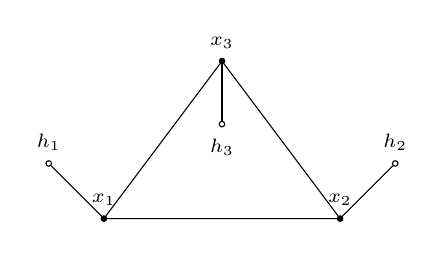
\begin{tikzpicture}[scale=1,
every label/.append style={font=\scriptsize},
point/.style = {draw, circle, fill=black, minimum size=2pt,inner sep=0pt},
root/.style={circle,fill=red!40, inner sep=2pt},
leaf/.style={circle,fill=green!40!black, inner sep=2pt}
]
\def\vertdist{.6}
\def\hordist{.7}
\node[point,label={[above]$x_1$}] (A) at (0,0) {};
\node[point,label={[above]$x_2$}] (B) at (3,0) {};
\node[point,label={[above]$x_3$}] (C) at (1.5,2) {};
\node[point,style={fill=white},label={[above]$h_1$}] (AA) at ($(A)+(-.7,.7)$) {};
\node[point,style={fill=white},label={[above]$h_2$}] (BB) at ($(B)+(.7,.7)$) {};
\node[point,style={fill=white},label={[below,yshift=-3pt]$h_3$}] (CC) at ($(C)+(0,-.8)$) {};
\draw (A) -- (B) node[midway, below] {$\Prpg$}-- (C)  node[midway, right] {$\Prpg$} -- (A)  node[midway, left] {$\Prpg$};
\draw (A) -- (AA);
\draw (B) -- (BB);
\draw (C) -- (CC);
\end{tikzpicture}}
\parbox{3cm}{$\begin{multlined}\scriptstyle\int_{x_1, x_2, x_3}\Prpg(x_1,x_2)\Prpg(x_2,x_3)\Prpg(x_3,x_1)\\ \scriptstyle h_1(x_1)h_2(x_2)h_3(x_3)\end{multlined}$}\vspace{.5cm}
\parbox{5.7cm}{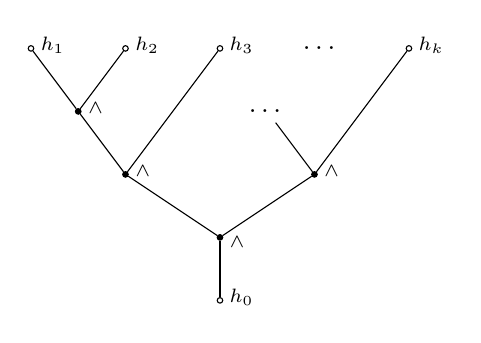
\begin{tikzpicture}[scale=1,
every label/.append style={font=\scriptsize},
point/.style = {draw, circle, fill=black, minimum size=2pt,inner sep=0pt},
]
\def\vertdist{.8}
\def\hordist{.6}
\node[point,style = {fill = white},label={[right] $h_0$}] (R) at (0,0) {};
\node[point, label={[right,yshift=-1mm] $\wedge$}] (RU) at ($(R) + (0,\vertdist)$) {};
\node[point, label={[right] $\wedge$}] (RUL) at ($(RU) + (-2*\hordist,\vertdist)$) {};
\node[point, label={[right] $\wedge$}] (RUR) at ($(RU) + (2*\hordist,\vertdist)$) {};
\node[point, label={[right] $\wedge$}] (RULL) at ($(RUL) + (-1*\hordist,1*\vertdist)$) {};
\coordinate (RULR) at ($(RUL) + (\hordist,\vertdist)$);
\coordinate (RURR) at ($(RUR) + (\hordist,\vertdist)$);
\node[point, style = {fill = white}, label={[right] $h_1$}] (RULLL) at ($(RULL) + (-1*\hordist,1*\vertdist)$){};
\node[point, style = {fill = white},label={[right] $h_2$}] (RULLR) at ($(RULL) + (1*\hordist,1*\vertdist)$) {};
\node[point, style = {fill = white}, label={[right] $h_3$}] (RULRR) at ($(RULR) + (1*\hordist,1*\vertdist)$) {};
\node[point, style = {fill = white}, label={[right] $h_k$}] (RURRR) at ($(RURR) + (1*\hordist,1*\vertdist)$) {};
\node[] (RURRL) at ($(RURR) + (-1*\hordist,1*\vertdist)$) {\ \,\dots};
\node (RURL) at ($(RUR) + (-\hordist,\vertdist)$) {\dots};
\draw (R) edge (RU); 
\draw (RU) -- (RUL) node[below,midway,shift={(-1.5mm,1mm)}] {$\Htp$}; 
\draw (RUL) -- (RULL) node[below,midway,shift={(-2mm,2mm)}] {$\Htp$}; 
\draw (RULL) edge (RULLL);
\draw (RULL) edge (RULLR);
\draw (RUL) edge (RULRR);
\draw (RU) -- (RUR) node[below,midway,shift={(2mm,2mm)}] {$\Htp$};
\draw (RUR) edge (RURL);
\draw (RUR) edge (RURRR);
\end{tikzpicture}}
\parbox{3cm}{
$\begin{multlined} 
\scriptstyle\langle h_0, \wedge \circ (\Htp \otimes \Htp)\circ (\wedge \otimes \wedge)\circ (\Htp \otimes \Id \otimes \dotsb  \otimes \Id)\\
 \scriptstyle\circ (\wedge \otimes \Id \otimes \dotsb \otimes \Id)(h_1, h_2, h_3, \dots, h_k)\rangle
\end{multlined}$}
\let\Prpg\OldPrpg
\let\Htp\OldHtp
\end{frame}

\begin{frame}{Effective Hochschild IBL-infinity chain model}
$\Implies$ $\BVOp^{\PMC} = \hat{\OPQ}^{\PMC}_{110}  +  \hbar \hat{\OPQ}_{210}^\PMC + \sum_{l\ge 2, g\ge 0} \hat{\OPQ}^{\PMC}_{1lg} \hbar^{l+g-1}$ on $\Fun(\BCyc \Harm)$ \\ 
\begin{itemize}
\item $\BVOp^{\PMC}\BVOp^{\PMC} = 0$ $\Equiv$ $(\CDBCyc \Harm,\OPQ_{klg}^\PMC)$ \emph{quantum co-$\LInfty$-algebra with Drinfeld compatible Lie bracket $\OPQ_{210}^\PMC = \OPQ_{210}$.}
\end{itemize}\pause\vspace{.3cm}
\emphbf{New invariant of $\mathbf{M}$:} htpy class $[(\CDBCyc \HDR, \OPQ_{klg}^\PMC)]$. What data?\\\pause\vspace{.3cm}
Recall: \emph{Kontsevich-Soibelman} $(\DR,\Dd,\wedge)$ $\xrightarrow{\AInfty-h.t.}$ $(\HDR,(m_k))$
\begin{itemize}
\item $[(\HDR, m_k)]_{\AInfty}$ topological invariant containing rational homotopy theory for $1$-connected $M$.
\item $m_k = \sum I(\text{trees})$ depends on $(\DR,\Dd,\wedge)$ and $\color{blue}\Htp$, not $\color{blue}\Prpg$, nor $\langle\cdot,\cdot\rangle$
\item $\OPQ_{110}^\PMC = \Hd_{\AInfty}^*$, \rlap{$\Hd_{\AInfty}(\omega_1\dotsc\omega_k) = \sum\limits_{c,i} \pm m_i(\omega_c \dotsc \omega_{c+i-1}) \dotsc\omega_{c+k}$}
\end{itemize}\pause
\vspace{.3cm}
$[(\CDBCyc \HDR, \OPQ_{klg}^\PMC)]$ depends on $(\DR,\Dd,\wedge,\langle\cdot,\cdot\rangle)$ as \emph{Poincar\'e DGA} because $\Prpg$ is needed to evaluate graphs with circles.
% We can choose either homotopy class of quantum co-$L_\infty$ algebra or of $\IBLInfty$. The former is finer because the condition on a co-$\LInfty$ algebra is stronger.
\end{frame}



\begin{frame}[fragile]{Contribution to $\mathbf{\OPQ_{120}^\PMC(\psi): \BCyc \Harm \otimes \BCyc\Harm \rightarrow \R}$}
\begin{center}
\def\BddMin{.2}
\def\BddMaj{.4}
\def\HorLen{2}
\def\PMCVert{1}
\def\PantsVert{2}
\def\PantsPlunge{.5}
\newcommand{\BddSurf}[6][0]{
% #1 rotation (the optional argument)
% #2 is the center, e.g., C1 or 0:1
% #3 is the major semiaxis
% #4 is the minor semiaxis
% #5 is the style of the upper half
% #6 is the style of the lower half
\draw[#5,rotate=#1] ([shift=(0:{#3} and {#4})]#2) arc (0:180:{#3} and {#4});
\draw[#6,rotate=#1] ([shift=(180:{#3} and {#4})]#2) arc (180:360:{#3} and {#4});
%
}
\hspace{-1.5cm}\begin{tikzpicture}[scale=1.3]
\tikzset{point/.style = {draw, circle, fill=black, minimum size=2pt,inner sep=0pt}}
\coordinate (C1) at (0,0);
\coordinate (CC) at ($(C1) + (\HorLen,0)$);
\coordinate (CV) at ($(C1) + (.5*\HorLen,\PMCVert)$);

\coordinate (C2) at ($(CC) + (.5*\HorLen,-\PantsVert)$);
\coordinate (CP) at ($(CC) + (.5*\HorLen,-\PantsPlunge)$);
\coordinate (C3) at ($(CC) + (\HorLen,0)$);
 
\BddSurf{C1}{\BddMaj}{\BddMin}{dotted}{}
\BddSurf{C2}{\BddMaj}{\BddMin}{dotted}{}
\BddSurf{C3}{\BddMaj}{\BddMin}{}{}
\BddSurf{CC}{\BddMaj}{\BddMin}{dotted}{dotted}

\draw ([shift={(\BddMaj,0)}]C1) to[out=90,in=180] ([shift={(0,-\BddMaj)}]CV);
\draw ([shift={(0,-\BddMaj)}]CV) to[out=0,in=90] ([shift={(-\BddMaj,0)}]CC);
\draw ([shift={(-\BddMaj,0)}]CC) to[out=-90,in=90] ([shift={(-\BddMaj,0)}]C2);
\draw ([shift={(\BddMaj,0)}]C2) to[out=90,in=-90] ([shift={(\BddMaj,0)}]C3);
% Lower countour

\draw ([shift={(-\BddMaj,0)}]C1) to[out=90,in=180] ([shift={(0,\BddMaj)}]CV);
\draw ([shift={(0,\BddMaj)}]CV) to[out=0,in=90] ([shift={(\BddMaj,0)}]CC);
\draw ([shift={(\BddMaj,0)}]CC) to[out=-90,in=180] (CP);
\draw (CP) to[out=0,in=-90] ([shift={(-\BddMaj,0)}]C3);
% Upper contour


\BddSurf[90]{CV}{\BddMaj}{\BddMin}{blue,dashed,thick}{blue,thick}
% The joint

\draw[red,thick] ([shift=(45:{\BddMin} and {\BddMaj})]CV) to[out=0,in=95] ([shift=(-40:{\BddMaj} and {\BddMin})]CC) to[out=-85,in=180] ([shift={(0,.-.25*\PantsPlunge)}]CP) to[out=0,in=-90] ([shift=(-140:{\BddMaj} and {\BddMin})]C3);
% The identity line


%START: Inputs from C1
\draw ([shift=(-60:{\BddMaj} and {\BddMin})]C1) to[out=90,in=180] ([shift=(-20:{\BddMin} and {\BddMaj})]CV);

\draw ([shift=(-110:{\BddMaj} and {\BddMin})]C1) to[out=90,in=180] ([shift=(20:{\BddMin} and {\BddMaj})]CV);

\draw[dashed] ([shift=(125:{\BddMaj} and {\BddMin})]C1) to[out=80,in=180] ([shift=(145:{\BddMin} and {\BddMaj})]CV);
%END: Inputs from C1

%START: Inputs from C2
\draw ([shift=(245:{\BddMaj} and {\BddMin})]C2) to[out=90,in=-80] ([shift=(240:{\BddMaj} and {\BddMin})]CC) to[out=100,in=0] ([shift=(-50:{\BddMin} and {\BddMaj})]CV);

\draw[dashed] ([shift=(110:{\BddMaj} and {\BddMin})]C2) to[out=90, in=-85] ([shift=(90:{\BddMaj} and {\BddMin})]CC) to[out=95, in=15] ([shift=(190:{\BddMin} and {\BddMaj})]CV);

\draw ([shift=(-60:{\BddMaj} and {\BddMin})]C2) to[out=90, in=-110] ([shift=(-40:{\BddMaj} and {\BddMin})]C3);

\draw[dashed] ([shift=(70:{\BddMaj} and {\BddMin})]C2) to[out=90, in=-90] ([shift=(80:{\BddMaj} and {\BddMin})]C3);
%END: Inputs from C2

\node[point] at ([shift=(-140:{\BddMaj} and {\BddMin})]C3) {};
\node[point] at ([shift=(190:{\BddMin} and {\BddMaj})]CV) {};

\node[point] at ([shift=(45:{\BddMin} and {\BddMaj})]CV) {};
\node[point] at ([shift=(-50:{\BddMin} and {\BddMaj})]CV) {};
\node[point] at([shift=(20:{\BddMin} and {\BddMaj})]CV) {};
\node[point] at ([shift=(-20:{\BddMin} and {\BddMaj})]CV) {};
\node[point] at ([shift=(145:{\BddMin} and {\BddMaj})]CV) {};

\node[label={[yshift=.1cm] $\psi$}] at (C3) {};
%\node[label={[yshift=-.9cm] $\omega_1$}] at (C1) {};
%\node[label={[yshift=-.9cm] $\omega_2$}] at (C2) {};
\node[label={[yshift=-.7cm] $\scriptstyle\color{red}\mathrm{T}$}] at (CP) {};
\node at ([shift={(0,-\BddMin)}]CV) {};

% External labels at the first boundary component
\node[point,style={fill=white},label={[below,yshift=-.1cm,xshift=.1cm] $\scriptstyle h_{13}$}] at ([shift=(-60:{\BddMaj} and {\BddMin})]C1) {};
\node[point,style={fill=white},label={[below,yshift=-.1cm,xshift=-.1cm] $\scriptstyle h_{12}$}] at ([shift=(-110:{\BddMaj} and {\BddMin})]C1) {};
\node[point,style={fill=white},label={[below,yshift=+.1cm,xshift=-.6cm] $\scriptstyle h_{11}$}] at ([shift=(125:{\BddMaj} and {\BddMin})]C1) {};

% External labels at the second boundary component
\node[point,style={fill=white},label={[below,xshift=-.1cm,yshift=-.1cm] $\scriptstyle h_{22}$}] at ([shift=(245:{\BddMaj} and {\BddMin})]C2) {};
\node[point,style={fill=white},label={[left,xshift=-.4cm] $\scriptstyle h_{21}$}] at ([shift=(110:{\BddMaj} and {\BddMin})]C2) {};
\node[point,style={fill=white},label={[below,xshift=.1cm,yshift=-.1cm] $\scriptstyle h_{23}$}] at ([shift=(-60:{\BddMaj} and {\BddMin})]C2) {};
\node[point,style={fill=white},label={[right,xshift=.4cm] $\scriptstyle h_{24}$}] at ([shift=(70:{\BddMaj} and {\BddMin})]C2) {};


% Internal labels of vertices
\node[label={[above,yshift=-.01cm] $\scriptstyle x_1$}] at ([shift=(145:{\BddMin} and {\BddMaj})]CV) {};
\node[label={[above,yshift=-.05cm,xshift=.1cm] $\scriptstyle x_2$}] at ([shift=(45:{\BddMin} and {\BddMaj})]CV) {};
\node[label={[right,xshift=-.07cm,yshift=-.18cm] $\scriptstyle x_3$}] at ([shift=(20:{\BddMin} and {\BddMaj})]CV) {};
\node[label={[right,yshift=-.2cm,xshift=-.1cm] $\scriptstyle x_4$}] at ([shift=(-20:{\BddMin} and {\BddMaj})]CV) {};
\node[label={[below,yshift=-.22cm] $\scriptstyle x_5$}] at ([shift=(-50:{\BddMin} and {\BddMaj})]CV) {};
\node[label={[left,yshift=-.2cm,xshift=.1cm] $\scriptstyle x_6$}] at ([shift=(190:{\BddMin} and {\BddMaj})]CV) {};
\node[font=\footnotesize] (ZZ) at ([shift={(0,-5ex)}]CV) {$\color{blue}\Prpg$};
\end{tikzpicture}
\let\OldPrpg\Prpg
\renewcommand{\Prpg}{{\color{blue}\OldPrpg}}
$\begin{multlined}
\scriptstyle \sum_{a,b}\sum_{c=1}^4 \pm  {\color{red}\mathrm{T}}^{ab} \psi(e_a  h_{2,c+2}  h_{2,c+3})  \Bigl(\int_{x_1 x_2 x_3 x_4 x_5 x_6} \Prpg(x_1,x_2)\Prpg(x_2,x_3)\Prpg(x_3,x_4)\\
\scriptstyle\Prpg(x_4,x_5)\Prpg(x_5,x_6)\Prpg(x_6,x_1)\bigl( h_{11}(x_1) h_{12}(x_3)
h_{13}(x_4)\bigr)\bigl(e_b(x_2)  h_{2,c}(x_6)  h_{2,c+1}(x_5)\bigr)\Bigr)
\end{multlined}$
\let\Prpg\OldPrpg
\end{center}
\end{frame}

\begin{frame}{Vanishing result}
\begin{theorem}[Vanishing for 1-connected manifolds $\mathbf{\neq \Sph{2}}$]
$\exists{\color{blue}\Prpg}$: $\HDR^1=0$ $\Implies$ \parbox[t]{7cm}{$\OPQ_{110}^\PMC = \Hd_{\AInfty}^*$, $\OPQ_{210}^\PMC=\OPQ_{210}$, $\OPQ_{120}^\PMC = \OPQ_{120}$ and $\OPQ_{klg}^\PMC = 0$ otherwise.}
\end{theorem}\pause
\begin{proof}
\parbox[b]{5cm}{\centering
%auto-ignore
\begin{tikzpicture}[scale=.7]
\tikzset{point/.style = {draw, circle, fill=black, minimum size=2pt,inner sep=0pt}}
\def\dist{5.5}
\def\startangle{90}
\def\leglength{1.2}
\def\dashpart{0.5}

\coordinate[point] (A) at (0,0);

\path (A) -- +(\startangle:\dashpart*\leglength) coordinate (A11) -- +(\startangle:\leglength) coordinate (A12);
\path (A) -- +(\startangle+120:\dashpart*\leglength) coordinate (A21) -- +(\startangle+120:\leglength) coordinate (A22);
\path (A) -- +(\startangle+240:\dashpart*\leglength) coordinate (A31) -- +(\startangle+240:\leglength) coordinate (A32);

\draw (A) -- (A12) node[point,style={fill=white},label={0:$1$}] {};
\draw (A) -- (A22) node[point,style={fill=white},label={$\omega$}] {};
\draw (A) -- (A31); \draw[dashed] (A31) -- (A32);
\end{tikzpicture}\\
$\int_x {\color{blue}\Prpg}(x,y)\omega(x) = 0$
}
\parbox[b]{5cm}{\centering
\begin{tikzpicture}[scale=.7]
\tikzset{point/.style = {draw, circle, fill=black, minimum size=2pt,inner sep=0pt}}
\def\dist{5.5}
\def\startangle{90}
\def\leglength{1.2}
\def\dashpart{0.5}
\coordinate[point] (B) at (0,0);
\path (B) -- +(\startangle:\dashpart*\leglength) coordinate (B11) -- +(\startangle:\leglength) coordinate (B12);
\path (B) -- +(\startangle+120:\dashpart*\leglength) coordinate (B21) -- +(\startangle+120:\leglength) coordinate (B22);
\path (B) -- +(\startangle+240:\dashpart*\leglength) coordinate (B31) -- +(\startangle+240:\leglength) coordinate (B32);

\draw (B) -- (B12) node[point,style={fill=white},label={0:$1$}] {};
\draw (B) -- (B21); \draw[dashed] (B21) -- (B22);
\draw (B) -- (B31); \draw[dashed] (B31) -- (B32);
\end{tikzpicture} \\
$\int_x {\color{blue}\Prpg}(x,y){\color{blue}\Prpg}(x,z) = 0$
} \\[.3cm]
$\Implies$ strong degree restriction $\deg(\omega_i)\ge 2$. \qedhere
\end{proof}\pause
\vspace{.3cm}
\begin{itemize}
\item $M$ geometrically formal $\Implies$ $\Hd_{\AInfty} = \Hd$.
\end{itemize}

\end{frame}

\begin{frame}{Role of formality}
\begin{itemize}
\item \emph{Formality} $:\Longleftrightarrow$ \parbox[t]{7cm}{structure on $\DR$ and the induced structure on $\HDR$ are weakly homotopy equivalent}\pause
\item \emph{$\IBLInfty$-formality:} $(\CDBCyc \HDR, \OPQ_{klg}^\PMC) \overset{\text{whe}}{\sim} (\CDBCyc\HDR,\Hd,\OPQ_{210},\OPQ_{120})$
\end{itemize}\pause
\vspace{.3cm}
\begin{conjecture}[Formality conjecture]
$\HDR^1 = 0$: $\DGA$-formality $\Implies$ $\IBLInfty$-formality.
\end{conjecture}
\begin{itemize}\pause
\vspace{.3cm}
\item Observation: $(\DR,\Dd,\wedge,\langle\cdot,\cdot\rangle) \overset{\text{whe}}{\sim} (\HDR,\wedge,\langle\cdot,\cdot\rangle)$ as Poincar\'e $\DGA$'s iff as $\DGA$'s $\Implies$ study Poincar\'e duality models of Poincar\'e $\DGA$'s and functoriality of $\dIBL$-construction.
\end{itemize}
% Not every whe of DGA's lifts to whe of PDGA's.
\end{frame}


\begin{frame}[fragile]{Thank you!}
\begin{center}
\def\baselist{{0,1.8,3.2}}
\def\hghtlist{{1.8,1.5,1}}
\def\wghtlist{{6,4,2}}
\def\trnkwght{.5}
\def\trnkhght{1.2}
\begin{tikzpicture}

% Trunk
\draw[fill=brown,draw=black] (-.5*\trnkwght,0)--(.5*\trnkwght,0)--(.5*\trnkwght,-\trnkhght)--(-.5*\trnkwght,-\trnkhght)--cycle;

% Tree
\foreach \i in {0,1,2}
{
% Floors
\draw[fill=ForestGreen,draw=green] ($(-.5*\wghtlist[\i],\baselist[\i])$) to[out=-10,in=-170] ($(.5*\wghtlist[\i],\baselist[\i])$) to[out=135,in=-45] ($(0,\baselist[\i]+\hghtlist[\i])$) to[out=-135,in=45] cycle;
%Balls
\node[circle,draw=yellow,fill=red,thick, minimum size=2mm] at ($(-.5*\wghtlist[\i],\baselist[\i])$) {};
\node[circle,draw=yellow,fill=red,thick, minimum size=2mm] at ($(.5*\wghtlist[\i],\baselist[\i])$) {};
}

% Star
\node at ($(0,\hghtlist[2]+\baselist[2])$) [star,fill =Dandelion,minimum size=1cm] {};
\end{tikzpicture}\\
\Huge \emphbf{Merry Christmas!}
\end{center}
\end{frame}

\end{document}
